\documentclass{article}

% if you need to pass options to natbib, use, e.g.:
%     \PassOptionsToPackage{numbers, compress}{natbib}
% before loading neurips_2026

% The authors should use one of these tracks.
% Before accepting by the NeurIPS conference, select one of the options below.
% 0. "default" for submission
\usepackage[preprint]{neurips_2026}
% the "default" option is equal to the "main" option, which is used for the Main Track with double-blind reviewing.
% 1. "main" option is used for the Main Track
%  \usepackage[main]{neurips_2026}
% 2. "position" option is used for the Position Paper Track
%  \usepackage[position]{neurips_2026}
% 3. "eandd" option is used for the Evaluations & Datasets Track
 % \usepackage[eandd]{neurips_2026}
% 4. "creativeai" option is used for the Creative AI Track
%  \usepackage[creativeai]{neurips_2026}
% 5. "sglblindworkshop" option is used for the Workshop with single-blind reviewing
 % \usepackage[sglblindworkshop]{neurips_2026}
% 6. "dblblindworkshop" option is used for the Workshop with double-blind reviewing
%  \usepackage[dblblindworkshop]{neurips_2026}
% 7. "education" option is used for the Education Track
%  \usepackage[education]{neurips_2026}


% After being accepted, the authors should add "final" behind the track to compile a camera-ready version.
% 1. Main Track
 % \usepackage[main, final]{neurips_2026}
% 2. Position Paper Track
%  \usepackage[position, final]{neurips_2026}
% 3. Evaluations & Datasets Track
 % \usepackage[eandd, final]{neurips_2026}
% 4. Creative AI Track
%  \usepackage[creativeai, final]{neurips_2026}
% 5. Workshop with single-blind reviewing
%  \usepackage[sglblindworkshop, final]{neurips_2026}
% 6. Workshop with double-blind reviewing
%  \usepackage[dblblindworkshop, final]{neurips_2026}
% Note. For the workshop paper template, both \title{} and \workshoptitle{} are required, with the former indicating the paper title shown in the title and the latter indicating the workshop title displayed in the footnote.
% For workshops (5., 6.), the authors should add the name of the workshop, "\workshoptitle" command is used to set the workshop title.
% \workshoptitle{WORKSHOP TITLE}
% 7. Education Track
% \usepackage[education, final]{neurips_2026}

% "preprint" option is used for arXiv or other preprint submissions
 % \usepackage[preprint]{neurips_2026}

% to avoid loading the natbib package, add option nonatbib:
%    \usepackage[nonatbib]{neurips_2026}

\usepackage[utf8]{inputenc} % allow utf-8 input
\usepackage[T1]{fontenc}    % use 8-bit T1 fonts
\usepackage{hyperref}       % hyperlinks
\usepackage{url}            % simple URL typesetting
\usepackage{booktabs}       % professional-quality tables
\usepackage{amsfonts}       % blackboard math symbols
\usepackage{nicefrac}       % compact symbols for 1/2, etc.
\usepackage{microtype}      % microtypography
\usepackage{xcolor} 
% colors
\usepackage[preprint]{neurips_2026}
\usepackage{amsmath,amssymb,amsthm,mathrsfs,mathtools,amsfonts,physics,bm,bbm,booktabs, gensymb}
\usepackage{subcaption}

% Note. For the workshop paper template, both \title{} and \workshoptitle{} are required, with the former indicating the paper title shown in the title and the latter indicating the workshop title displayed in the footnote. 
\title{Capturing non-Markovian effects in weather prediction models}


% The \author macro works with any number of authors. There are two commands
% used to separate the names and addresses of multiple authors: \And and \AND.
%
% Using \And between authors leaves it to LaTeX to determine where to break the
% lines. Using \AND forces a line break at that point. So, if LaTeX puts 3 of 4
% authors names on the first line, and the last on the second line, try using
% \AND instead of \And before the third author name.


\author{
}


\begin{document}


\maketitle


\begin{abstract}
  
\end{abstract}



\section{Introduction to the architecture}
Turbulent flows are known as a notoriously difficult framework for numerical simulations. One of the common method in such simulations is the \textit{direct numerical simulations} (DNS) that discretize the Navier-Stokes equation to a space and time grid and then simulate directly. Such discretizations, however require a very fine grid resolution scaling as $N_{\textrm{grid}} \sim \left(Re\right)^{\alpha}$ with $\alpha \sim 2.05 $ \cite{yang2021grid}. Insufficient small-scale resolution may leave mean dissipation and enstrophy approximately converged while substantially underestimating high-order moments of velocity gradients, dissipation, and enstrophy, as well as the tails of velocity-gradient distributions and statistics involving second velocity derivatives \cite{DonzisResolutionEffects}.
 While this becomes expensive, a variety of models that regularize the equations on a larger scale, introducing proper dissipative terms at the cost of short time accuracy \cite{Wilson1996Review}. Another approach consists in keeping coarse-grained scales, without non-controlled dissipative approximation, but at a cost of keeping the non-Markovian memory terms \cite{YenTingLinMZ2021,de2026data}.

In this article, we explore the potential of such methods for a weather prediction models.
\subsection{Two Hybrid architectures}
For our study, we select a Markovian pretrained model, and intentionally learn a non-Markovian kernel for a temporal interaction. In this article, we introduce and study a hybrid GraphCast-Mamba architecture, that captures non-Markovian effects. This architecture, is shown schematically in Fig.~\ref{fig:GC_Mamba}. 

\paragraph{GraphCast}
For a baseline Markovian model we use a DeepMind checkpoint of the GraphCast model. This is a graph neural network (GNN) model which operates on two grids - original lattitude-longitude grid, and the auxiliary mesh grid. The full model operates on a graph $\mathcal{G}(\mathcal{V}^{\textrm{G}},\mathcal{V}^{\textrm{M}},\mathcal{E}^{\textrm{G2M}},\mathcal{E}^{\textrm{M}},\mathcal{E}^{\textrm{M2G}})$, where $\mathcal{V}^{\textrm{G}}$ is the original lattitude-longitude grid containing the physical data, $\mathcal{V}^{\textrm{M}}$ is a much smaller mesh grid. The model first a first mapping $\mathcal{E}^{\textrm{M2G}}$ from grid-to-mesh, then $N$ ($N=16$ for resolution 0.25\degree GraphCast model) processor message passing steps $\mathcal{E}^{\textrm{M}}$ on a mesh grid and finally grid-to-mesh mapping $\mathcal{E}^{\textrm{G2M}}$ back to the original grid. Each node has the same dimension $W_{\textrm{GC}}$ (canonical GC value $W_{\textrm{GC}}=512$). The total number of mesh nodes $N_{\textrm{mesh}}$ is typically much smaller than the number of grid nodes $N_{\textrm{grid}}$.

\paragraph{Mamba}
Mamba is an attention-free sequence model based on selective state-space models (SSMs), designed to model long temporal dependencies with computation that scales linearly with sequence length \cite{gu2023Mamba}. A conventional continuous-time SSM maps an input sequence $x(t)$ to a latent memory state $h(t)$ according to
\begin{equation}
    \frac{d h(t)}{dt} = A h(t) + B x(t),
    \qquad
    y(t) = C h(t) + D x(t).
\end{equation}
Here, $A$ is a diagonal matrix that determines how quickly memory decays or evolves, $B$ and $C$ determines how new inputs are written into the state and readout from the state respectively, and $D$ provides a direct input-to-output skip connection. For a single SSM channel, each of the matrices have fixed dimension $d_{\textrm{state}}=16$ and $\Delta$ - is a scalar. If $A$, $B$, and $C$ are fixed, the same linear dynamical system is applied at every time step. For a discrete step size $\Delta$, its exact discretization is
\begin{equation}
    h_t = \bar{A} h_{t-1} + \bar{B}x_t,
    \qquad
    \bar{A} = \exp(\Delta A),
    \qquad
    \bar{B} = A^{-1}\left[\exp(\Delta A)-I\right]B.
\end{equation}

Mamba makes this SSM \emph{selective}: rather than using fixed input and readout matrices and a fixed step size, it computes $B_t$, $C_t$, and $\Delta_t$ from the current input. Thus, the model can decide which information to retain, overwrite, or expose at each time step.

In our model, Mamba operates independently on the temporal sequence of each GraphCast mesh node. Let $x_t^{\mathrm{in}}\in\mathbb{R}^{W_{\textrm{GC}}}$ denote the mesh latent feature at a given node and forecast step. A layer-normalized input is projected into two $d_{\textrm{inner}}$-dimensional branches (typically $d_{\textrm{inner}}=W_{\textrm{GC}}/4$),
\begin{equation}
    [\tilde{x}_t,z_t]
    =
    W_{\mathrm{in}}\operatorname{LN}(x_t^{\mathrm{in}}),
    \qquad
    \tilde{x}_t,z_t\in\mathbb{R}^{d_{\textrm{inner}}}.
\end{equation}
The first branch, $\tilde{x}_t$, supplies the SSM input. The second branch, $z_t$, is a learned output gate: it does not update the memory state directly, but controls how much of the SSM output is passed onward.

Before entering the SSM, $\tilde{x}_t$ is processed by a depthwise causal one-dimensional convolution with kernel width four:
\begin{equation}
    u_{t,d}
    =
    \operatorname{SiLU}
    \left(
        b^{\mathrm{conv}}_d
        +
        \sum_{k=0}^{d_{\textrm{conv}}-1}
        w^{\mathrm{conv}}_{d,k}\tilde{x}_{t-k,d}
    \right),
    \qquad d=1,\ldots, d_{\textrm{inner}},
\end{equation}
where $\operatorname{SiLU}(a)=a/(1+e^{-a})$. ``Depthwise'' means that each of the $d_{inner}$ channels has its own $d_{\textrm{conv}}$ learned convolution weights $w^{\mathrm{conv}}_{d,k}$ and does not mix with other channels at this stage. ``Causal'' means that $u_t$ depends only on the current input and the three previous inputs, never on future inputs. During autoregressive inference, the preceding three projected inputs are retained in a convolution cache, so this local temporal context continues across forecast calls.

The selective parameters are generated from $u_t$ by learned linear projections:
\begin{equation}
    [r_t,B_t,C_t] = W_xu_t,
    \qquad
    r_t\in\mathbb{R}^{d_t},
    \quad
    B_t,C_t\in\mathbb{R}^{d_{\textrm{state}}},
\end{equation}
\begin{equation}
    \Delta_t
    =
    \operatorname{softplus}(W_\Delta r_t+b_\Delta)
    \in\mathbb{R}^{d_{\textrm{inner}}}.
\end{equation}
\lh{($d_t=32,d_{state}=16$)}All matrices, vectors, convolution kernels, and biases in these equations are trainable parameters optimized end-to-end by gradient descent using the forecasting loss. In contrast, $B_t$, $C_t$, and $\Delta_t$ are not fixed parameters: they are input-dependent values generated anew at each time step from $u_t$. The softplus function ensures $\Delta_t>0$.

The continuous-time state matrix is diagonal and parameterized as
\begin{equation}
    A_{d,n}=-\exp(A_{\log,d,n}),
    \qquad
    d=1,\ldots,d_{\textrm{inner}},\quad n=1,\ldots,d_{\textrm{state}}.
\end{equation}
Because every element of $A$ is negative, the corresponding factor $\exp(\Delta_{t,d}A_{d,n})$ lies between zero and one, giving stable, decaying memory. The implementation uses the following selective recurrence:
\begin{equation}
    h_{t,d,n}
    =
    \exp\!\left(\Delta_{t,d}A_{d,n}\right)h_{t-1,d,n}
    +
    \Delta_{t,d}B_{t,n}u_{t,d}.
\end{equation}
The first term retains a scaled portion of the previous state, while the second writes the current input into memory. A small $\Delta_{t,d}$ gives slow decay and long memory; a large $\Delta_{t,d}$ gives faster decay and a stronger update from the current input.

The state is read out using the selective vector $C_t$ and a learned skip parameter $D$:
\begin{equation}
    s_{t,d}
    =
    \sum_{n=1}^{16} C_{t,n}h_{t,d,n}
    +
    D_d u_{t,d}.
\end{equation}
Finally, the gate branch $z_t$ modulates this readout, and the result is projected back to the $W_{\textrm{GC}}$-dimensional GraphCast latent space:
\begin{equation}
    o_t
    =
    W_{\mathrm{out}}
    \left[
        s_t\odot\operatorname{SiLU}(z_t)
    \right],
    \qquad
    x_t^{\mathrm{out}}=x_t^{\mathrm{in}}+o_t.
\end{equation}

Our main configuration uses an internal channel dimension of $128$, an SSM state dimension of $16$ per channel, a causal convolution width of $4$, and a rank-$32$ projection for $\Delta_t$. The SSM state $h_t$ and the three-token convolution cache persist separately for every batch element, mesh node, Mamba layer, and autoregressive forecast step.



\begin{figure}
    \centering
    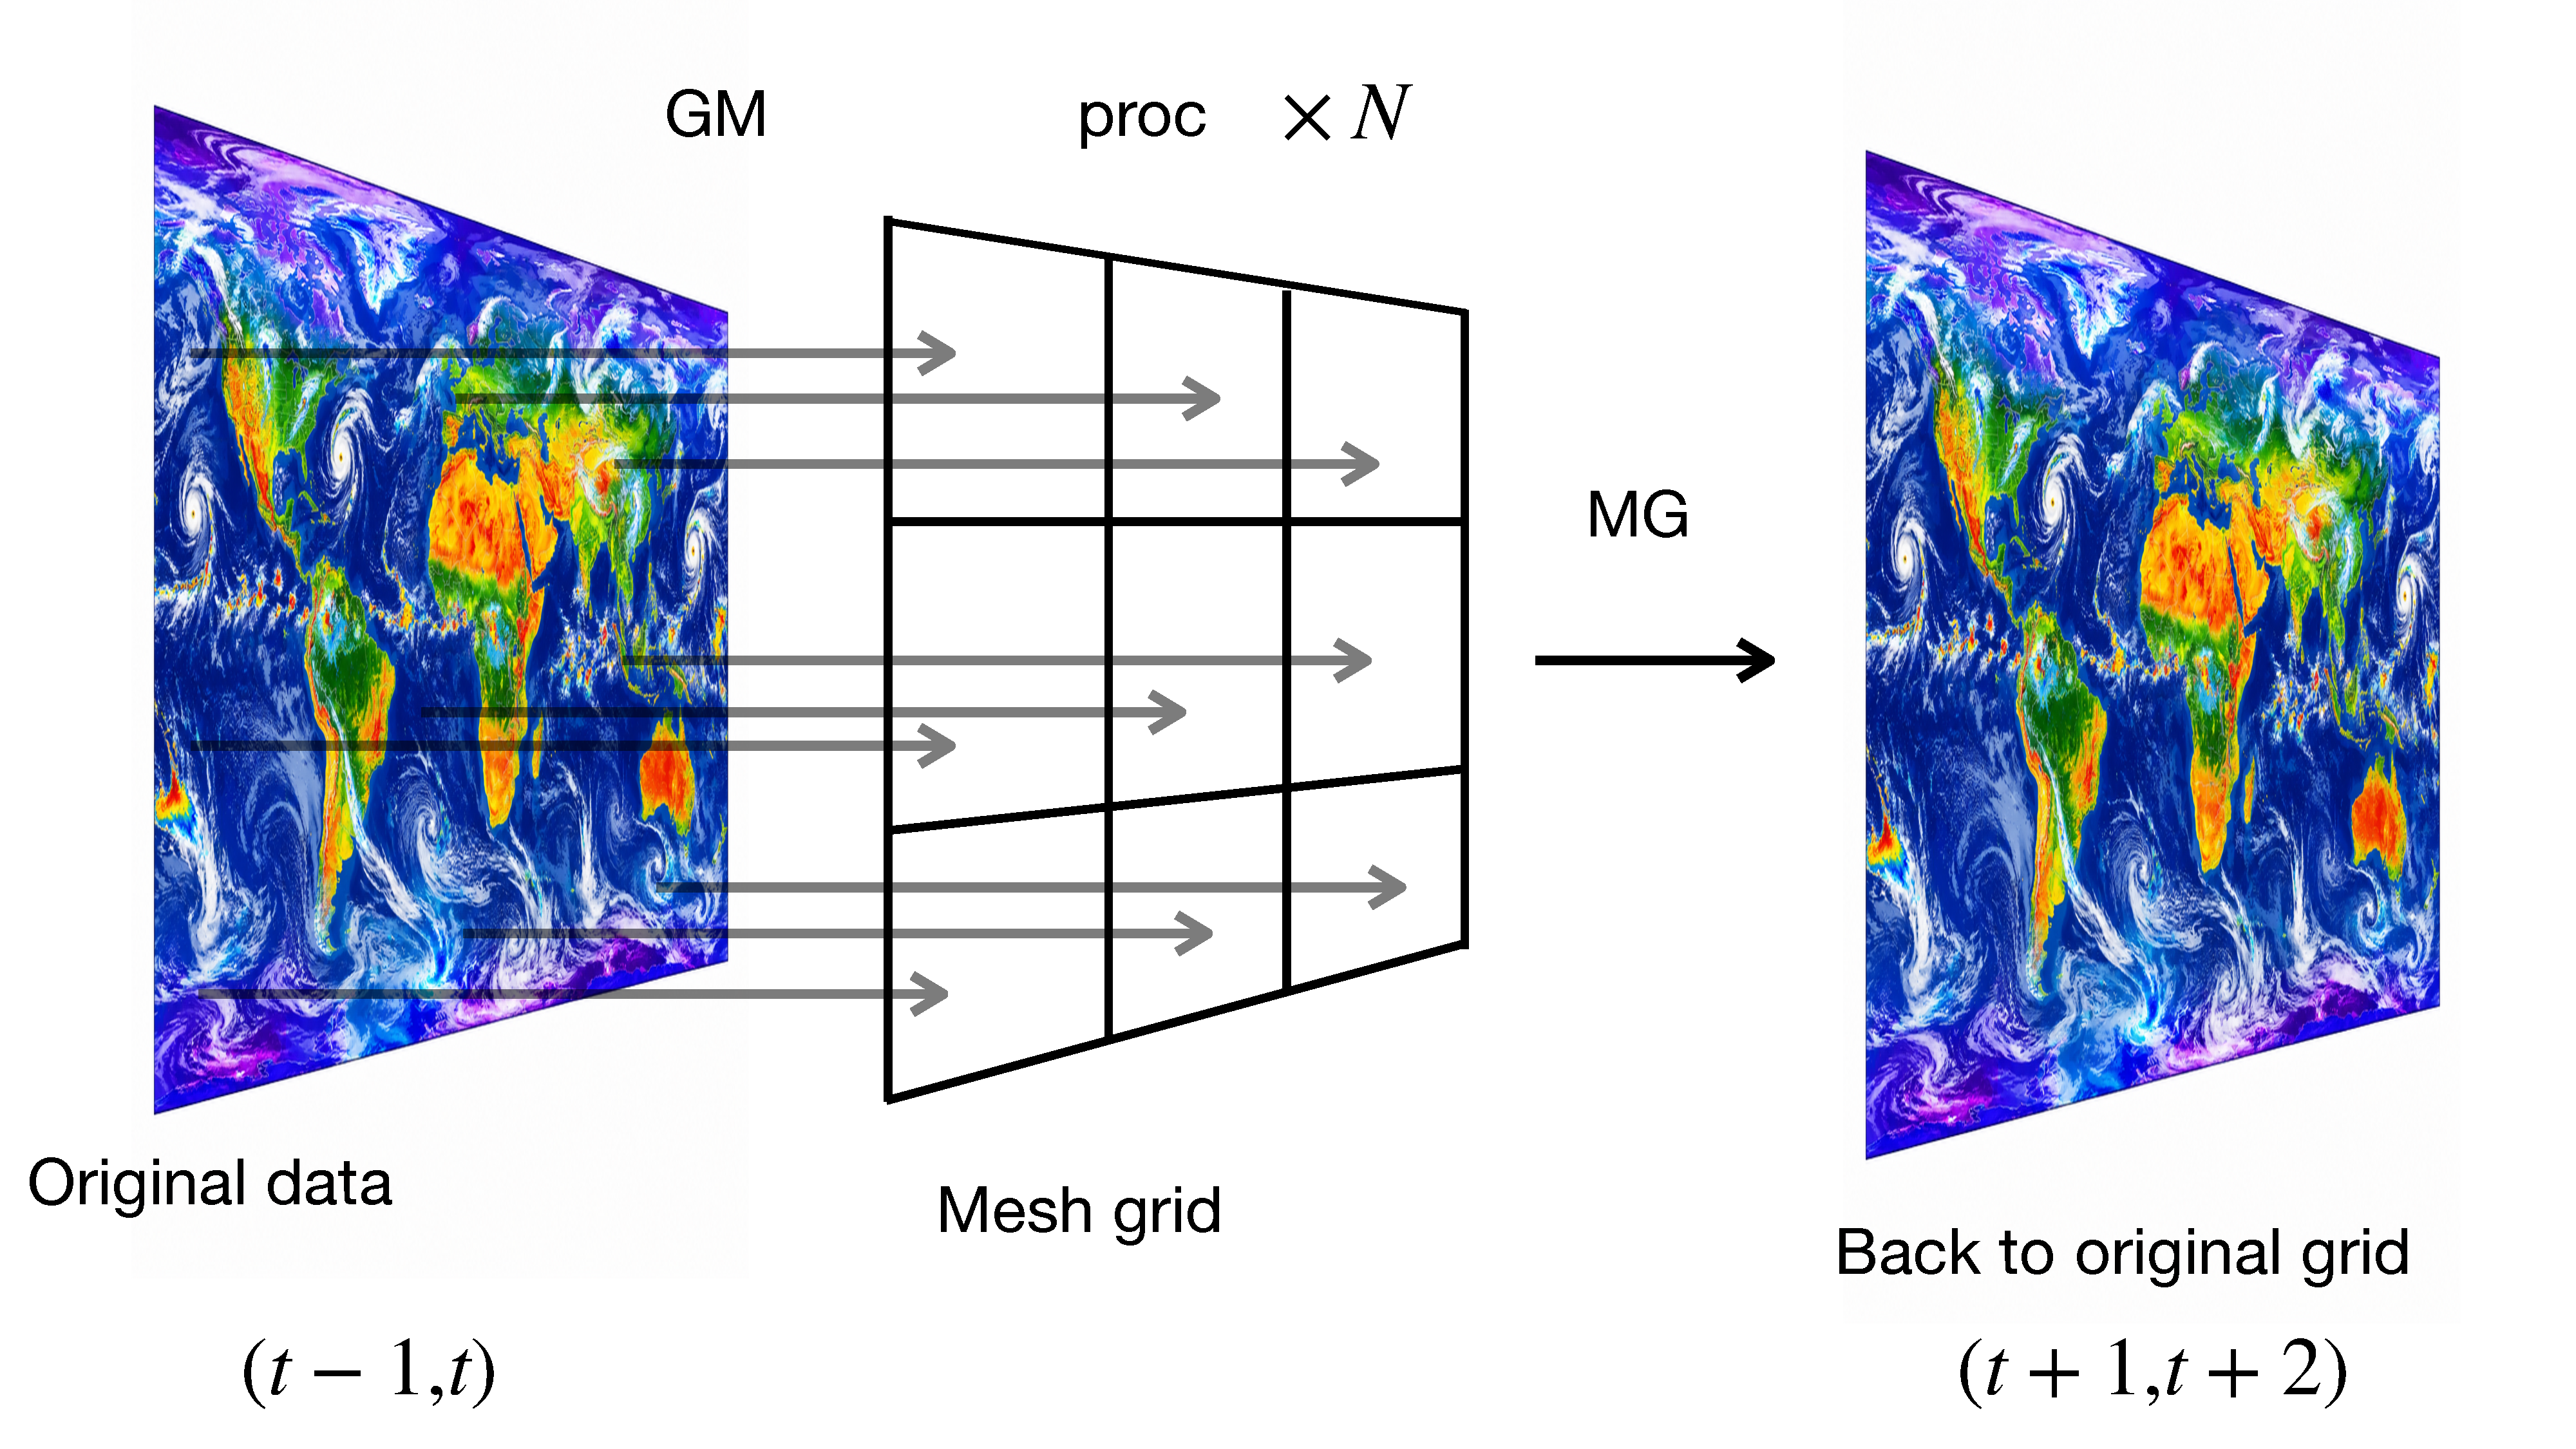
\includegraphics[width=0.9\linewidth]{Pics/GC.pdf}\\
    \subcaption[1]{Schematic GraphCast architecture, original data are projected to a mesh grid, and after the iteration of $N$ processor steps, projected back to the original grid.}
    \includegraphics[width=0.9\linewidth]{Pics/GC_Mamba.pdf}
    \caption{GraphCast-Mamba architecture, we additionally insert blocks of Mamba neural network, with a hidden state represented by a red dot. The dynamics of the hidden state, simulates the non-Markovian connection.}
    \label{fig:GC_Mamba}
\end{figure}

\paragraph{Additive and residual Mamba branches.}
We investigate two ways of combining Mamba with a pretrained GraphCast forecast. Let $G_{\theta}(X_t)$ denote the prediction of the pretrained GraphCast baseline from the meteorological input history $X_t$. In both cases, GraphCast provides a strong physical-spatial forecast, while Mamba provides temporally persistent information through its recurrent state. The final prediction is expressed as the baseline forecast plus a learned correction.

In the \textit{additive Mamba} formulation, Mamba is a separate correction branch, such that the final prediction $\hat{Y}_t=G_{\theta}(X_t)+c_t^{\mathrm{add}}$: is a linear combination of the GraphCast prediction and a shallow GraphCastMamba model trained separately.
\begin{equation}
    c_t^{\mathrm{add}}
    =
    M_{\phi}(Z_t;h_{t-1}),
    \qquad
    h_t
    =
    \operatorname{MambaStateUpdate}_{\phi}(Z_t,h_{t-1}),
\end{equation}

Here, $h_t$ is the persistent Mamba state, and $\phi$ denotes the trainable parameters of the Mamba branch. The baseline GraphCast model can remain frozen, so optimization learns only the additive correction. This construction is modular: GraphCast generates the main forecast, while Mamba learns the temporal component of the error that remains after the baseline prediction.

In the \textit{residual Mamba} formulation, Mamba is instead integrated into a trainable residual GraphCast head. The pretrained GraphCast backbone first provides mesh latent features $L_t$, and a residual graph neural network (GNN) further processes these features. Mamba blocks are inserted between GNN message-passing updates, allowing temporal memory to directly modify the evolving mesh representation:
\begin{equation}
    L_t^{(0)} = L_t,
    \qquad
    \widetilde{L}_t^{(k)}
    =
    \operatorname{GNN}^{(k)}_{\phi}
    \left(L_t^{(k-1)}\right),
\end{equation}
\begin{equation}
    L_t^{(k)}
    =
    \widetilde{L}_t^{(k)}
    +
    \operatorname{Mamba}^{(k)}_{\phi}
    \left(\widetilde{L}_t^{(k)};h_{t-1}^{(k)}\right),
    \qquad k=1,\ldots,K.
\end{equation}
The resulting features are decoded into a residual forecast,
\begin{equation}
    c_t^{\mathrm{res}}
    =
    \operatorname{Decode}_{\phi}\left(L_t^{(K)}\right),
    \qquad
    \hat{Y}_t
    =
    G_{\theta}(X_t)
    +
    c_t^{\mathrm{res}}.
\end{equation}

The essential difference is therefore where the temporal model acts. Additive Mamba predicts a correction in a separate branch and combines it with GraphCast only at the output. Residual Mamba injects the Mamba update into the residual GNN latent representation, so temporal memory can interact with graph message passing before the correction is decoded. In both approaches, the Mamba state is carried forward across autoregressive forecast steps, enabling the correction to depend on information accumulated over the preceding forecast trajectory.
\section{Numerical results}
\subsection{Mamba vs resolution}

Initially, we noted a non-monotonic dependence of the model acccuracy, depending on the initial grid resolution. However, later we observed that the shape of this curve is highly influenced by the amount of training data see Fig.~\ref{fig:res_sweep}. Interestingly, addition of Mamba branch improves the high resolution models, an probably demands less data to learn.

\begin{figure}
    \centering
    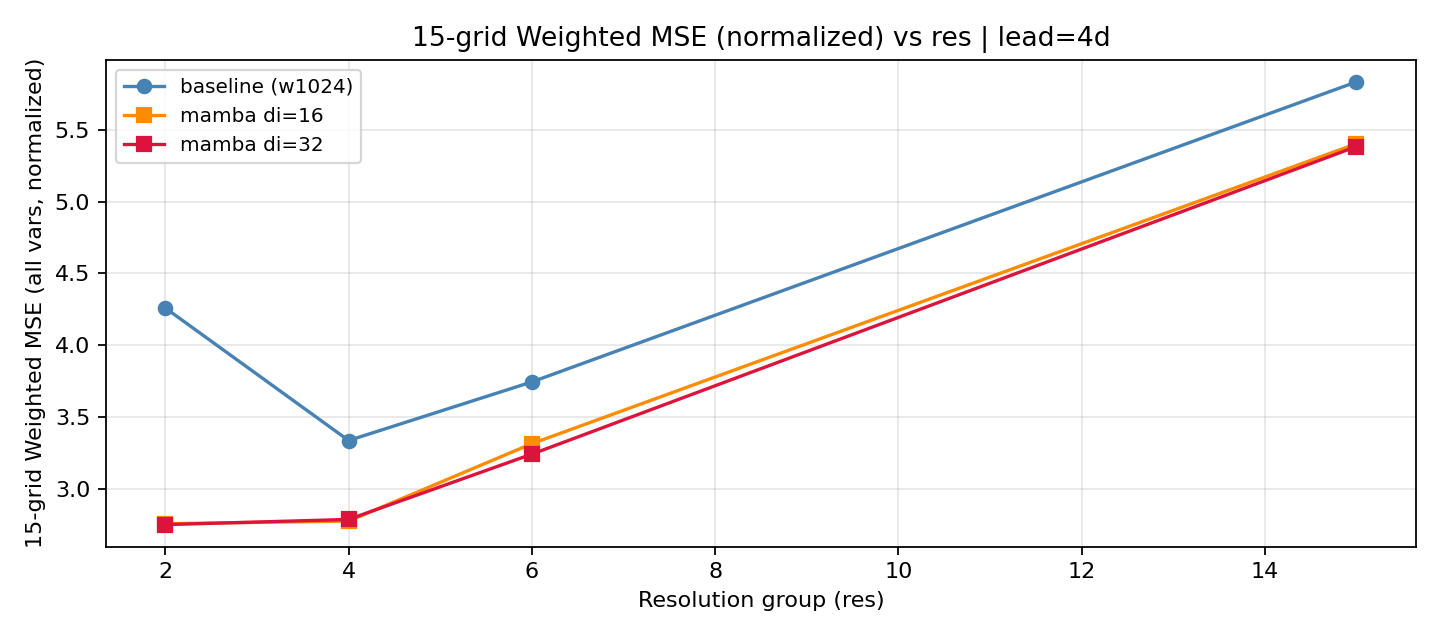
\includegraphics[width=0.49\linewidth]{Graphs/Vanilla_GC_res_Sweep.png}
    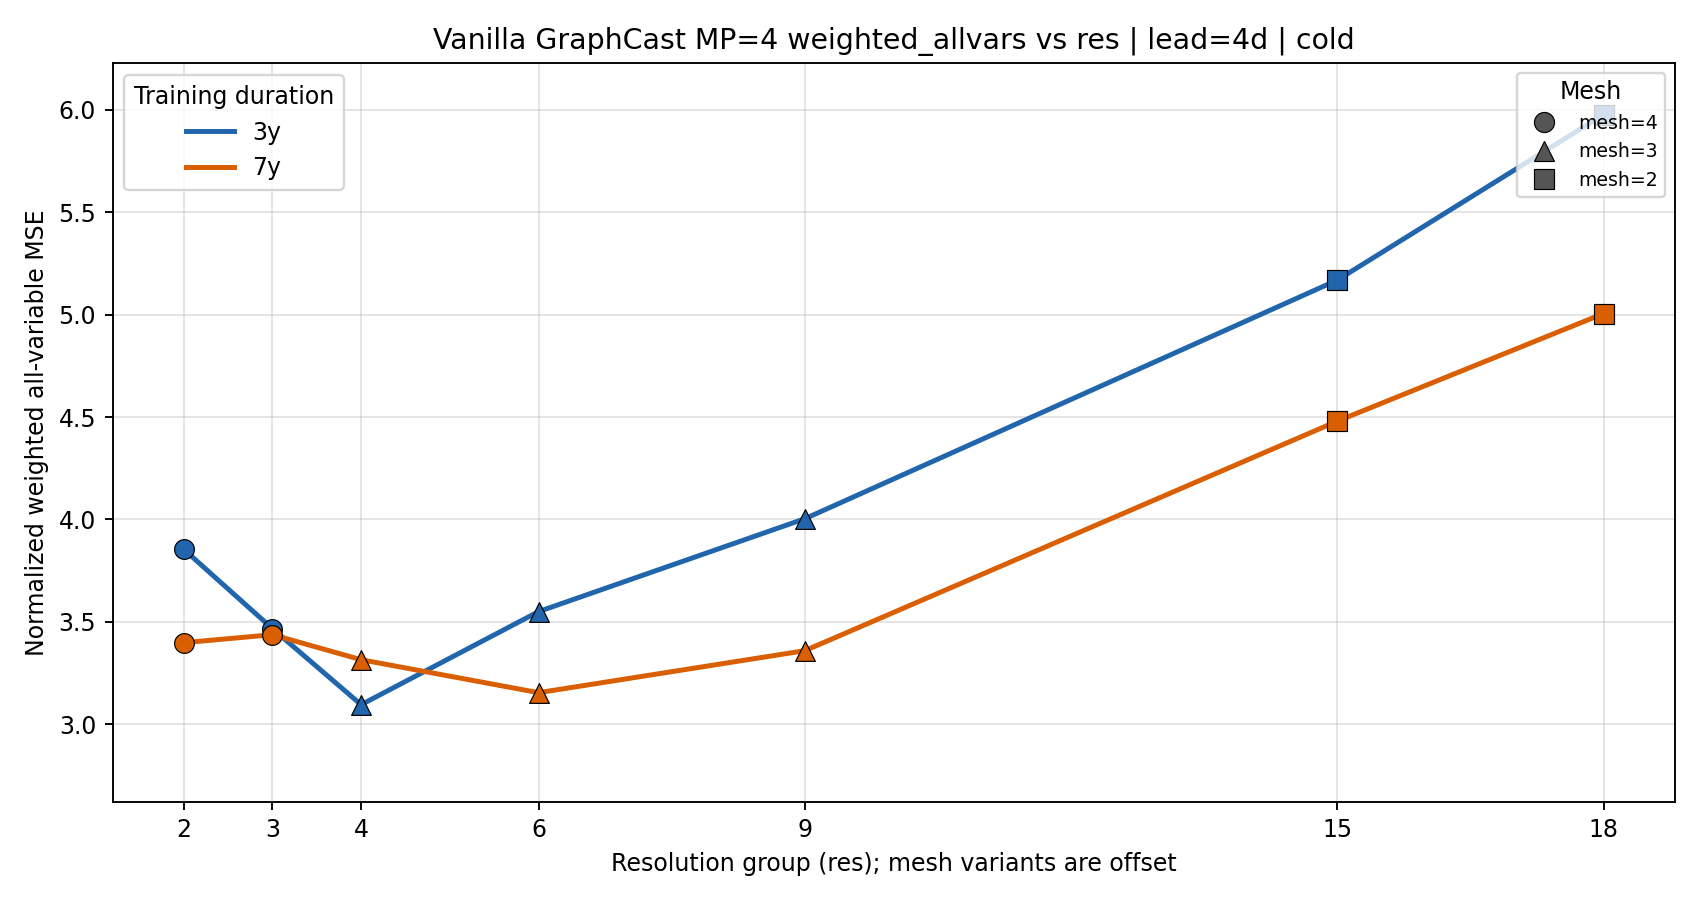
\includegraphics[width=0.4\linewidth]{Graphs/Vanilla_GC_Res_sweep_3_7_y.png}
    \caption{Comparison of models with different resolutions and the size of training dataset.}
    \label{fig:res_sweep}
\end{figure}
\subsection{Small resolution models}
First, we perform a study of resolution 2\degree models. Here, we pretrain the standard small sized GraphCast models, with only 6 message passing steps, and width $W=512$. On top of it, we learn both the additive and residual Mamba blocks. During this training, we optimize the error at $K=12$ timesteps, which is equal to a 4 day forecast that is generated autoregressively (AR) by feeding the previous output to the next input, with continuous updates of the mamba state.

We explored two possibilities of this AR unrolling: the so-called open and closed loops. In the open loop formulation we don't feed the full prediction to the next step, but only a part generated by the baseline GraphCast model -- this enforces model to be closer to an original GraphCast, and prevents instabilities related to an unphysical grow of Mamba part. The other strategy is the closed loop, which feeds back the full prediction. We also noted, that, especially for closed loop, eval loss behaves quite randomly, this is a signal that additional use of SWA technique, migh help a lot. The results are provided in Fig.~\ref{fig:add_mamba_res2}. 

Similarly, we trained the residual Mamba model, with the closed loop only. The comparison of the two models are plotted in Fig.~\ref{fig:res_add_Mamba}

\begin{figure}
    \centering
    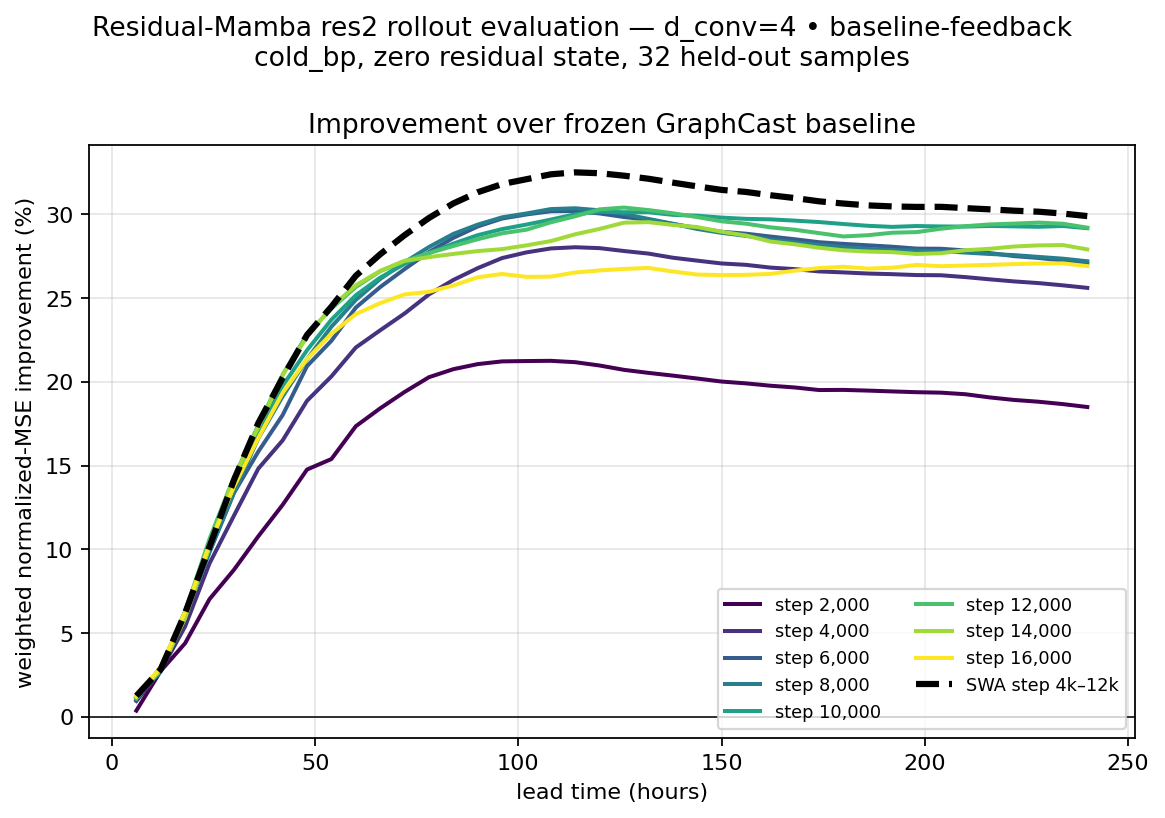
\includegraphics[width=0.45\linewidth]{Graphs/addMamba_res2_open.png}
    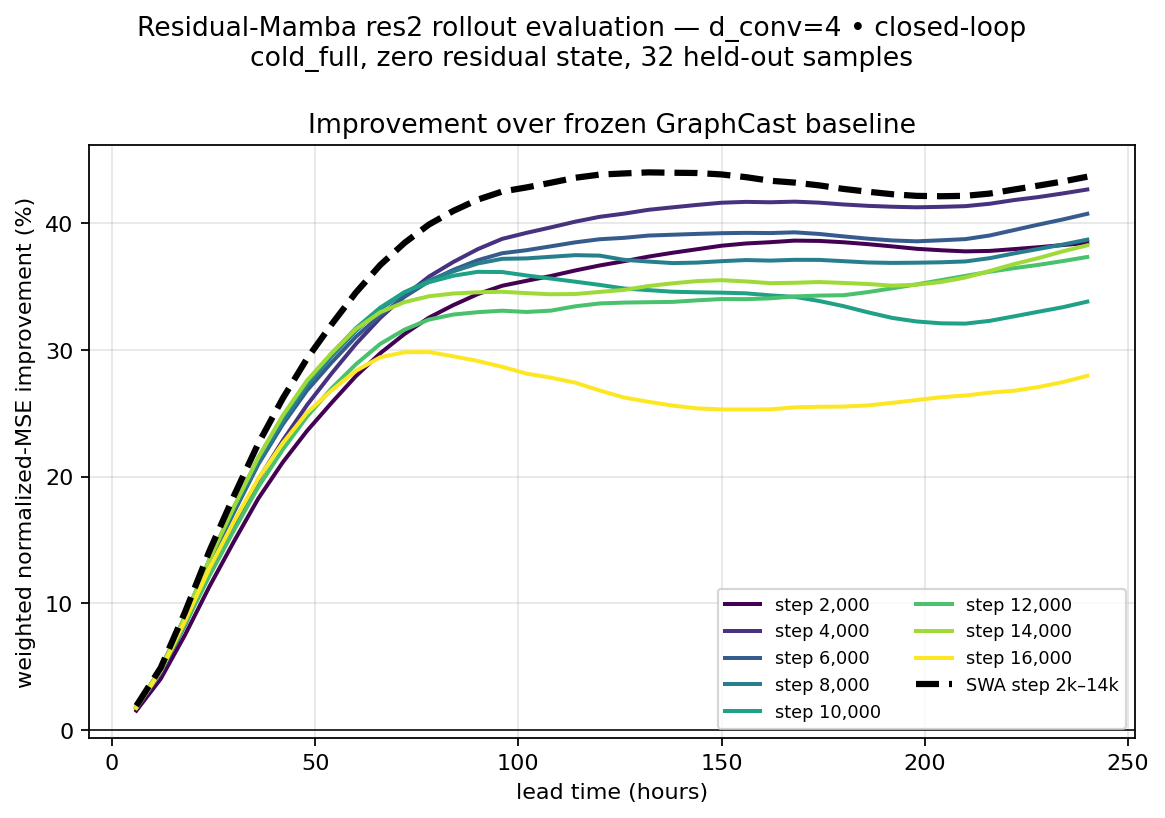
\includegraphics[width=0.45\linewidth]{Graphs/addMamba_res2_closed.png}
    \caption{Additive Mamba branch, a comparison of open loop model, and closed loop, both with and without SWA. $d_{inner}=16, d_{state}=16$}
    \label{fig:add_mamba_res2}
\end{figure}
\begin{figure}
    \centering
    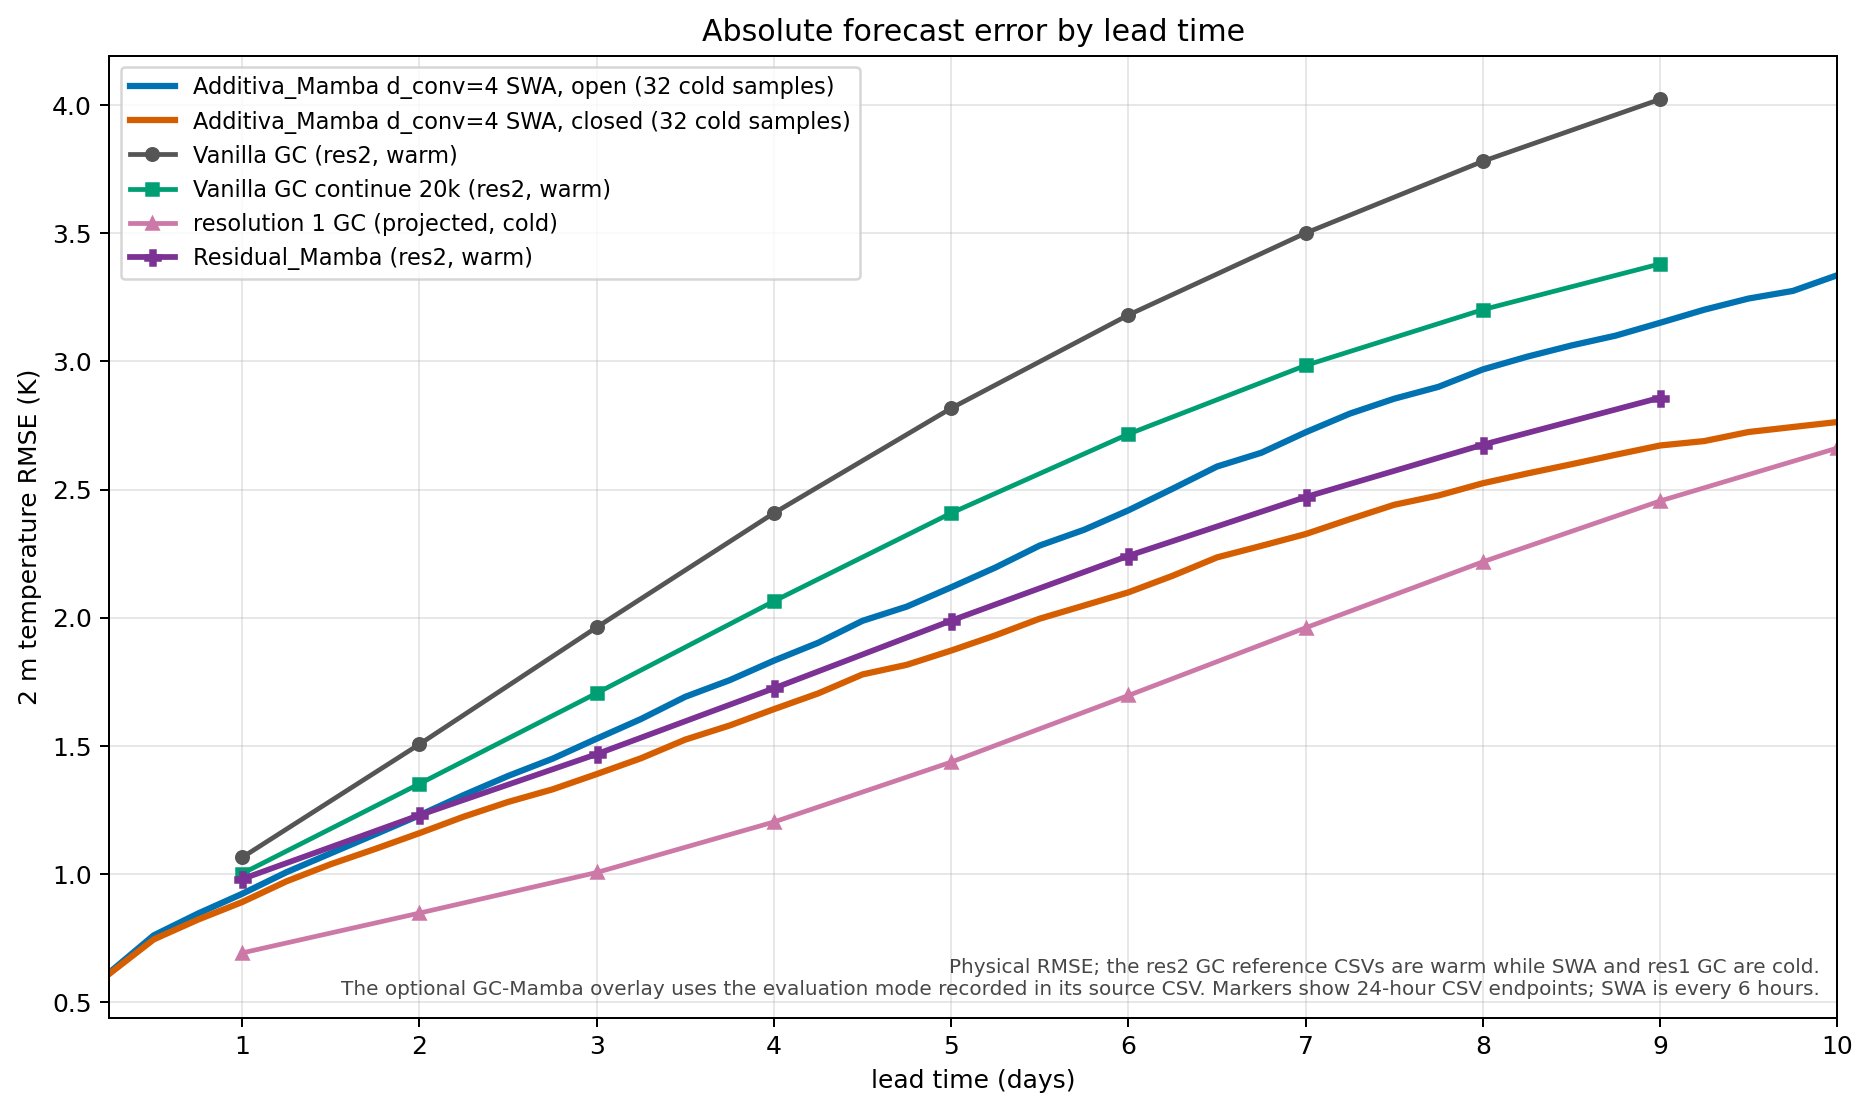
\includegraphics[width=0.90\linewidth]{Graphs/ResMamba_res2.png}
    \caption{Comparison of residual and additive Mamba models, the much larger DeepMind checkpoint GraphCast small is provided for comparison}
    \label{fig:res_add_Mamba}
\end{figure}


\subsection{resolution 1\degree}
For the resolution 1\degree model, we take the DeepMind trained GraphCast small checkpoint, and train the additive Mamba branch. The numerical result is provided in Fig.~\ref{fig:res1_add_Mamba}. We see that the addition of an additive Mamba branch can significantly improve the long-time accuracy, without compromising short times.

\begin{figure}
    \centering
    \includegraphics[width=0.9\linewidth]{Graphs/add_Mamba.png}
    \caption{Comparison of the GraphCast small (resolution 1\degree) model, and the additive Mamba model trained on top of it. The Results of GraphCast large (0.25\degree) are shown for comparison.}
    \label{fig:res1_add_Mamba}
\end{figure}

\section{ToDo:}
\subsection{Why larger Mamba models do not give any improvement?}
\subsection{Compare residual and additive branch more for resolution 2\degree and also resolution 1\degree}
\subsection{Train GraphCasr large (0.25\degree resolution)}
\bibliographystyle{plainnat}
\bibliography{bib}




\appendix
\section{Resolution Projection}
\section{Stochastic Weighted Average}
ref~\cite{izmailov2019averagingweightsleadswider}
\end{document}